% !TEX root = ../main.tex

\chapter{Background}
This chapter introduces to bitcoin, the world of cryptocurrency and marketplaces. It describes as well 
what is a proof of solvency, and some of its evolution and current state.

\section{Bitcoin}
%Andreas M. Antonopoulos somewhere
Bitcoin is recognized as the world's first successful cryptocurrency and decentralized digital currency. 
The goal of Bitcoin is to allow financial transactions to be settled without the need of a financial institution.
Transactions can occur within 2 participants of the network in realtime, without any middleman. 
All transactions are settled on a public blockchain, which means that everything can be verified by everyone. 


\subsection{Transactions}
For every participant of the network, there is a public key,  a private key and a wallet address.
The public key is derived from the private key using elliptic curve multiplication, and the wallet address is derived from the public key using a hashing function.
Both are one way function, meaning you cannot derived the other way around.
The wallet address can be seen as a bank account number. When you send bitcoin to someone, you send it to their wallet address.
To be able to send some bitcoin, you need to sign your transaction. 
Since transactions are sent on the network, we need to make sure a transaction originates from the sender.
The way to do that is to sign your transaction. The digital signature is created from the transaction data and the private key, which is only known by the owner of the address.
The public key is then used to make sure that the signature originates from the right private key.
Sending a transaction is the easiest problem to solve. The real challenge is to keep track of who owns what, and to avoid the double spending problem.
The way to do that is to keep the history of every single transactions. 
Bitcoin is a blockchain. The blockchain is made of blocks, and the transactions are filling these blocks.


\subsection{Network}
The challenge of the network, is to have every single node agree on the transaction history. Nodes are computers connected to the network,
working on publishing new blocks. The nodes work together to agree on the order of transactions. Every new transaction is broadcaseed to all nodes.
The nodes puts the transactions into a block, and try to publish that block. In order to publish a block, each node need to solve a proof-of-work challenge.
When a node solves the challenge, it broadcasts the block to every nodes. The nodes accepts the block if all transactions are valid. Their is no formal
way of approving a new block. A node show its acceptance by starting to work on a new block using the hash of the accepted block as previous hash.
Some nodes might accept different blocks, depending on what time they received new blocks. To solve the issue of multiple chains, the longest chain is consideredto be the correct one. 
If two chains have the same length, nodes keep working on their respective chains untill one of the chains receive a new block, breaking the tie.


\subsection{Proof-of-work}
In order to submit a new block, a node have to find a hash with x number of leading 0 bits.
It is exponentially more difficult every time you add a zero. The way to have different hash values, is to change the block timestamp, and the nonce value.
The nonce value is there solely for that purpose. Once a block is published, you cannot change any value inside of it because the hash value would change.
You would need to redo all the work to find a new good hash. Older blocks are even more secured, because in order to change the 2nd to last block, you would need to redo the work
for the 2 latest blocks. This is the same for every block down the road. The longest chanin is determined by the greatest proof-of-work invest in it. If their is a majority of honest nodes,
that chain will grow up the fastest. The difficulty of the new block is determined by an average, in order to generate blocks at a steady pace.


\subsection{Merkle Tree}
Only the merkle root is stored in the block header. When a block is enough in the past, nodes start to only keep block headers in memory.
They do not keep the rest of the block. This is why the hash of a block is the hash of the block header, and not the whole block. To keep the integrity of the chain.
The merkle root is the top of the Merkle Tree. A merkle tree is a tree where the parent node is the hash of the child nodes.

\begin{figure}[ht!]
\centering
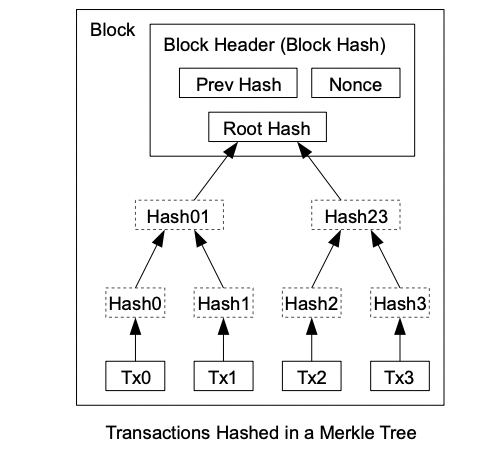
\includegraphics[width=90mm]{MerkleTree.png}
\caption{Bitcoin Merkle Tree \cite{N08}}
\label{overflow}
\end{figure}


\section{Marketplaces}
The best way to buy bitcoin for the first time is thourgh marketplaces. Marketplaces allow you to exchange money for bitcoin, but the bitcoin
you acquire in the process is not linked to a wallet address you own. It is in custody of the marketplace. In order to have possession of the bitcoins,
you need to enter a transfer request, where the bitcoin you own is sent to your wallet. Once you have bitcoins, you can transact on the network without needing
a 3rd party, unless you are running a node, you will need to trust a 3rd party, wheter it is a marketplace, or over the counter.

While the bitcoin you own is in custody of the marketplace, there is no way to see your bitcoin onchain. Marketplaces have many wallets, some are made public and some are not.
This is an inherent contradiction. Bitcoin was built to be transparent and public, without the need of a 3rd party to do a transaction.
The problem with no being able to track your bitcoin in a marketplace, is that you have no proof that the marketplace has enough bitcoin to reimburse
every client who has bitcoin in the marketplace.
However, this problem is being actively worked on. Marketplaces have begin to use proof of solvency (or proof of reserve) to show that they are solvent, but there is still a long way to go \cite{BPR}.
%Talk about FTX?


\section{Zero Knowledge}
Zero knowledge proofs is a proof that something is known, without revealing any informations. For instance,
the classic way of proving that you know the solution to an equation f(x), is to give the x that solves the equation.
However, with zero knoledge you are able to prove that you know the solution, without giving x. 
To construct a zero knowledge proof, you need to construct a proof that is sound and compelte. You also need your proof to be zero knowledge\cite{LZK}.

\begin{itemize}

    \item \textbf{Completeness}: If the statement is true, an honest verifier will be convinced by an honest prover.
    
    \item \textbf{Soundness}: If the statement is false, no dishonest prover can convince the honest verifier (except with some infinitysimal probability).
    
    \item \textbf{Zero-Knowledge}: If the statement is true,  a verifier learns nothing other than the fact that the statement is true. \cite{LC23}
    
    \end{itemize}


    \subsection{Non interactive proofs} 

Zero knowledge proofs were originaly designed as interactive, that is multiple rounds of interaction between the prover and the verifier \cite{GMR89}.
 leading to what are called interactive zero-knowledge proofs. An alternative model was then proposed where the verifier and prover use a 
 reference string that is shared during a trusted setup. Once we have the reference string, a single message is needed between the prover and the verifier.
 No rounds of interactions are needed. These are called noninteractive zero knowledge proofs.  \cite{BFM88} \cite{GMW91}


 \subsection{SNARKS} 
One of the recent advancement for non-interactive proofs is what is known as SNARK (non-interactive argument of knowledge).
This means a proof that is:
\begin{itemize}

    \item \textbf{Succinct}: the size of the proof is very small compared to the size of the witness.
    
    \item \textbf{Non-interactive}: No rounds of interactions between the prover and the verifier.

    \item \textbf{Argument}: Secured only for provers with bounded computational ressources, that is a dishonest prover with unlimited computational power could prove a wrong statement.

    \item \textbf{Knowledge-sound}: If the statement is true,  a verifier learns nothing other than the fact that the statement is true. \cite{NZ20}
    
    \end{itemize}

A SNARK can also be zero-knowedge. We call such proof a zk-SNARK.

\subsection{Arithmetic circuit} 
SNARKs use arithmetic circuits. An arithmetic circuit is a set gates, each assigned a distinct set of inputs corresponding to the numbers to be processed. 
These gates are configured to execute arithmetic operations such as addition, subtraction, multiplication, or division. The outputs of the gate circuit represent the digits of the resulting computation.

\begin{figure}[H]
    \centering
    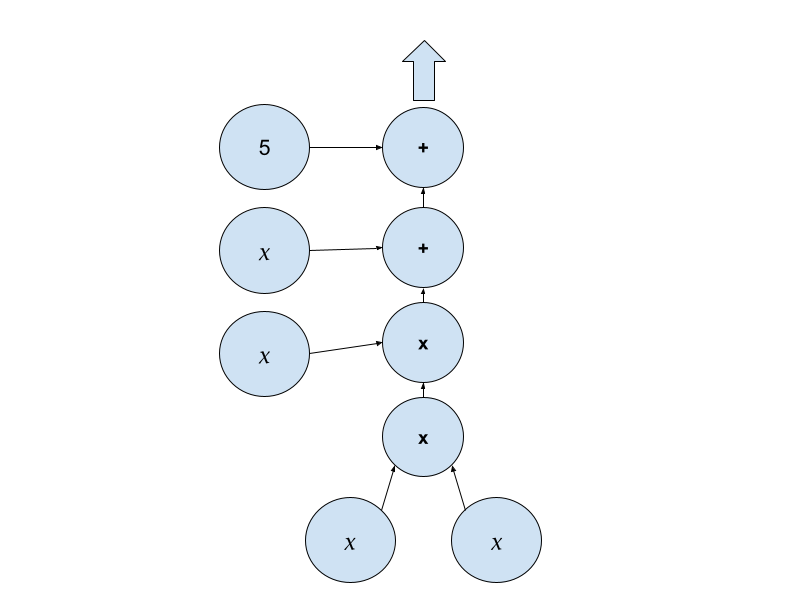
\includegraphics[width=60mm]{ArithmeticCircuit.png}
    \caption{General Arithmetic circuit \cite{ZKP23}}
    \label{overflow}
    \end{figure}

For SNARKs, the prover can create a proof, using the setup parameter, a private witness, and public input,
showing that the arithmetic circuit is equal to 0. That proof can be verified by the verifier using the stup parameter
and the public input.

\begin{figure}[H]
    \centering
    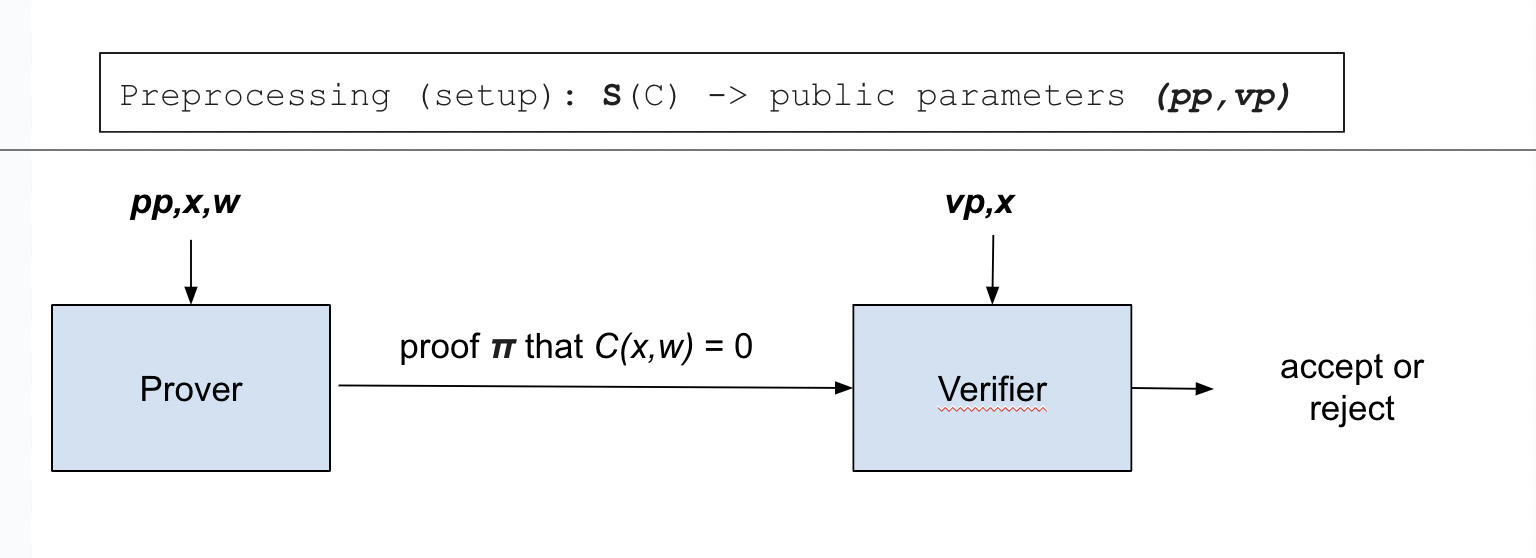
\includegraphics[width=130mm]{Circuit.png}
    \caption{Arithmetic circuit for SNARK \cite{ZKP23}}
    \label{overflow}
    \end{figure}

\begin{itemize}

    \item \textbf{S(C)}: Public parameters (pp,vp) for prover and verifier
    
    \item \textbf{P(pp,x,w)}: Proof $\pi$

    \item \textbf{V(vp,x,$\pi$)}: Accept or reject

    \item \textbf{C(x,w)}: Arithmetic circuit

    \item \textbf{w}: Private witness

    \item \textbf{x}: Public input
    
    \end{itemize}

%If STARK is mentionned later, define it here



\section{Proof of solvency}
%What is a proof of solvency
%History of papers
%What is wrong with Binance proof of solvency

 



